\section{Composite}

Esse padrão fornece uma estrutura de objetos organizados como uma 
árvore, representados através de uma hierarquia. Dessa forma, é 
possível tratar tanto o conjunto quanto os objetos individualmente, 
não sendo necessário conhecer todos os objetos pertencentes ao conjunto 
para tratar do mesmo.

Para alcançar isso, uma interface que representa um componente é 
implementada por uma classe "Folha", ou seja, um elemento não-composto 
e por uma classe Composite, ou seja, um elemento que também é um 
conjunto de outros elementos. Um Composite não sabe se os elementos 
que o compõem são também instâncias de Composite ou se são elementos 
folha, pois os elementos são apenas instâncias de Component.

\begin{figure}[htb]
	\caption{\label{fig_grafico}Estrutura do Composite}
	\begin{center}
	    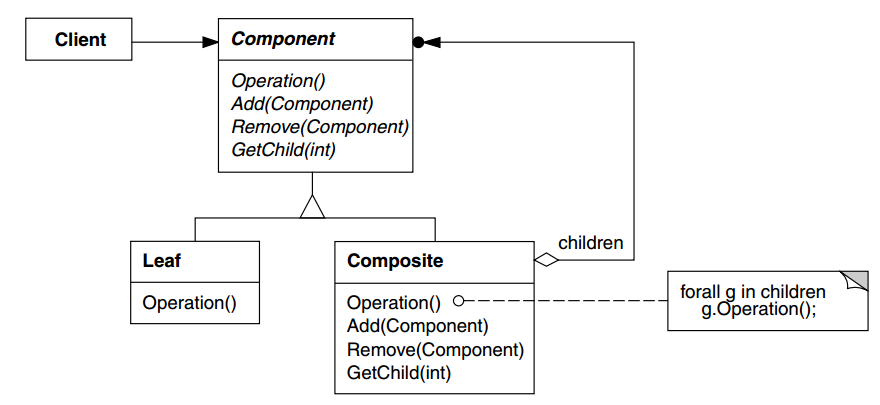
\includegraphics[scale=0.5]{5_padroes-contexto-funcional/5.2_estruturais/5.2.3_composite/diagram.png}
	\end{center}
\end{figure}

Exemplo Orientado a Objetos:

\begin{lstlisting}[caption={Composite Orientado a Objetos},label=oocomposite]



\end{lstlisting}

Contexto Funcional:



\begin{lstlisting}[caption={Composite Funcional},label=fpcomposite]
    

    
\end{lstlisting}